\section{Hodgking-Huxley equations}
\label{sec:Hodgking-Huxley}
The Hodgkin-Huxley equations~\cite{HodgkinHuxley1952} relate the difference in electric
potential across the cell membrane $V$ and gating variables $m, n$ and $h$
for ion channels to the stimulus intensity $I$ and temperature $T$, as
follows:
\begin{equation}
\label{eq:HodgkinHuxleyEquations}
\begin{cases}
\begin{aligned}
    \dot{V} &= -G(V, m, n, h)+I, \\
    \dot{m} &= \Phi(T)\left[(1-m) \alpha_{m}(V)-m \beta_{m}(V)\right], \\
    \dot{n} &= \Phi(T)\left[(1-n) \alpha_{n}(V)-n \beta_{n}(V)\right], \\
    \dot{h} &= \Phi(T)\left[(1-h) \alpha_{h}(V)-h \beta_{h}(V)\right],
\end{aligned}
\end{cases}
\end{equation}
where 
\begin{align*}
    \Phi(T) & = 3^{({T}-6.3) / 10}, \\
    G(V, m, n, h) & =\bar{g}_{\mathrm{Na}} m^{3}
    h\left(V-\bar{V}_{\mathrm{Na}}\right)+\bar{g}_{\mathrm{K}}
    n^{4}\left(V-\bar{V}_{\mathrm{K}}\right)+\bar{g}_{\mathrm{L}}\left(V-\bar{V}_{\mathrm{L}}\right).
\end{align*}
The equations modeling the variation of membrane permeability are:
\begin{align*}
    \alpha_{m}(V) =& \Psi\left(\frac{V+25}{10}\right), & \beta_{m}(V) &= 4 e^{V / 18}, \\
    \alpha_{n}(V) =& 0.1 \Psi\left(\frac{V+10}{10}\right), & \beta_{n}(V) &= 0.125 e^{V / 80}, \\
    \alpha_{h}(V) =& 0.07 e^{V / 20}, & \beta_{h}(V) &= \left(1+e^{(V+30) / 10}\right)^{-1},
\end{align*} with
\begin{equation*}
    \Psi(x) = \begin{cases}
        x /\left(e^{x}-1\right), & \text { if } x \neq 0, \\
        1, & \text { if } x=0.
    \end{cases}
\end{equation*}
The parameters $\bar{g}_{\text{ion}}$ and $\bar{V}_{\text{ion}}$ representing
maximum conductance and equilibrium potential for the ion were obtained from
experimental data by Hodgkin and Huxley, with the values given below:
\[
\begin{array}{lll}
\bar{g}_{\mathrm{Na}}=120 \mathrm{mS} / \mathrm{cm}^{2}, 
& \bar{g}_{\mathrm{K}}=36 \mathrm{mS} / \mathrm{cm}^{2}, 
& \bar{g}_{\mathrm{L}}=0.3 \mathrm{mS} / \mathrm{cm}^{2}, \\
\bar{V}_{\mathrm{Na}}=-115 \mathrm{mV},
& \bar{V}_{\mathrm{K}}=12 \mathrm{mV}, 
& \bar{V}_{\mathrm{L}}=10.599 \mathrm{mV}.
\end{array}
\]
The values of $\bar{V}_{\mathrm{Na}}$ and $\bar{V}_{\mathrm{K}}$ can be
controlled experimentally~\cite{HodgkinHuxley1952a,Jack1975ElectricCurrentFlow}.
The temperature is set to $T=6.3^{\circ}$.

It is easy to see that the equilibria of \cref{eq:HodgkinHuxleyEquations} can be
parametrized by $V$
\begin{equation*}
    \begin{aligned}
        I(V) &= G(V, m(V), n(V), h(V)) \\
        y(V) &= \alpha_y(V)/(\alpha_y(V)+\beta_y(V)),
    \end{aligned}
\end{equation*}
where $y\in\{m,n,h\}$, see also~\cite{Guckenheimer@1993}. By calculating the Jacobian $A$ of
\cref{eq:HodgkinHuxleyEquations} at the equilibrium, we can derive the
characteristic polynomial $\rho_A(\lambda)$. The equation $\rho_A(0)=0$ can be
solved analytically for $\bar V_K$. Using this solution for $\bar V_k$ and
plotting the curve $\rho'(0)$ reveals two potential candidates for Bogdanov--Takens
points. Inspecting the geometric multiplicity of these two points narrows the
possibilities down to the point
\begin{equation}
\label{eq:HodgkinHuxleyBTpoint}
\begin{pmatrix}
    V \\m \\n \\h \\ \bar V_k \\ I 
\end{pmatrix}
\approx
\begin{pmatrix}
-2.835463618170097 \\ 0.07351498630356315 \\ 0.361877602925177 \\ 0.494859128785482 \\
-4.977020454108788 \\ -0.06185214966177632
\end{pmatrix}.
\end{equation}  
Inspecting the coefficients of the normal form shows that
\[
a = 2.5515\cdot 10^{-5}, \qquad b =  -0.0075.
\] 
Thus, provided the transversality conditions are satisfied, we can use \MATCONT to
start continuation of the homoclinic orbits emanating from this point.

\begin{figure}
    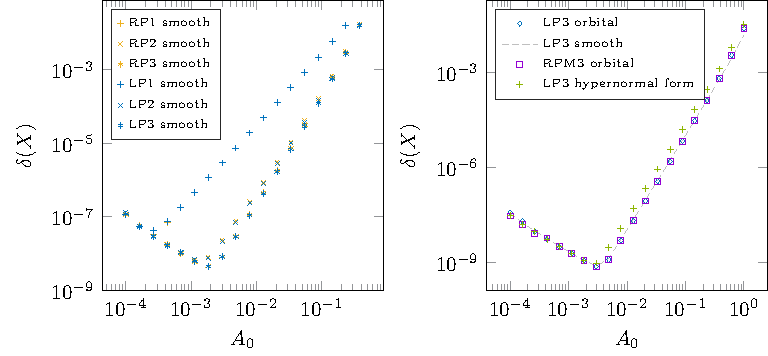
\includegraphics{\imagesdir/HodgkinHuxleyConvergencePlotFull.pdf}
    \caption{Convergence plot for the homoclinic predictors near the
    Bogdanov--Takens bifurcation \cref{eq:HodgkinHuxleyBTpoint} in the
    Hodgkin-Huxley equations \cref{eq:HodgkinHuxleyEquations}.}
    \label{fig:HodgkinHuxleyConvergencePlot}
\end{figure}

In \cref{fig:HodgkinHuxleyConvergencePlot} there are two log-log convergence
plots shown. In the left plot we compare the regular
perturbation method with the Lindstedt-Poincar\'e method. We see that compared
with the previous example, the Lindstedt-Poincare\'e method is slightly less
accurate than the regular perturbation method and the second-order.
Nevertheless, we clearly see that the order of convergence lifts from the
normal form to the two-dimensional center manifold in $\mathbb R^4$. In the
plot right we compare four different third approximations to the homoclinic
orbit
\begin{itemize}
    \item the Lindstedt-Poincar\'e method using the smooth orbital normal form
        (the blue diamond),
    \item the Lindstedt-Poincar\'e method using the smooth normal form
        (the dashed light gray line),
    \item the regular perturbation method using the smooth normal form
        (the pink square), 
    \item the Lindstedt-Poincar\'e method using the hyper-normal form
        (the green plus).
\end{itemize}

We see that both the Lindstedt-Poincar\'e method and the regular perturbation
method using the smooth orbital normal form are in perfect agreement with the
Lindstedt-Poincar\'e method using the smooth normal form. Only the homoclinic
predictor using the hyper-normal form is slightly less accurate.
